\section{Models}
In this work we took in consideration some models used in the state of the art, also adding some small modifications to make them fit better to our use case.
In particular, we focused on:
\begin{itemize}
    \item Menet for RPE;
    \item PoseNet and MapNet for APE.
\end{itemize}

\subsection{Menet}
MeNet is a model used for RPE. \Cref{fig:menet-structure} represents the structure of the model. The input of the network is a stack of two images, the goal of the model is to estimate the pose of the second image given the reference system fixed on the first one. The final prediction can be composed by 6 or 7 elements, this depends on the representation used for the rotation of the camera.
\begin{figure}
    \begin{center}
        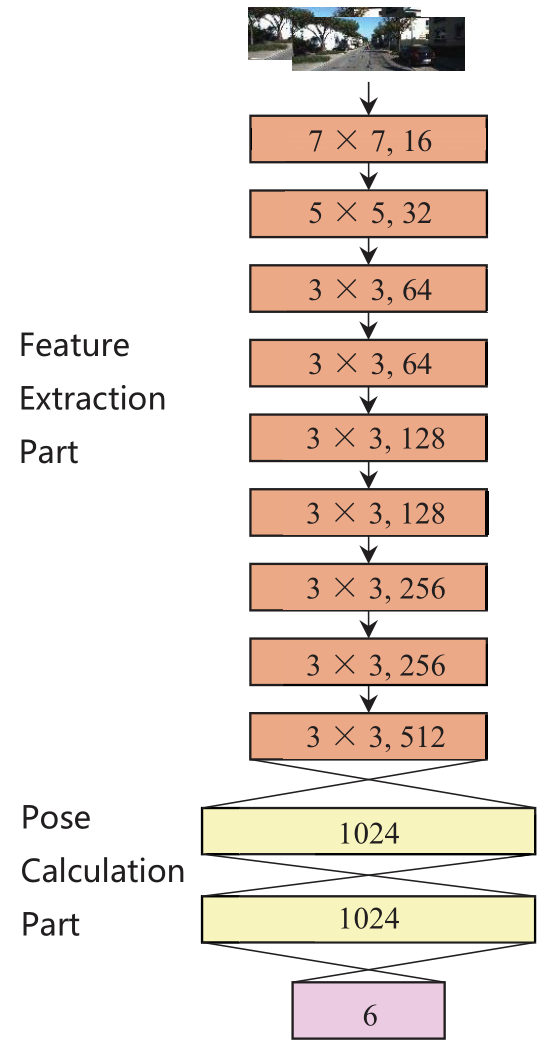
\includegraphics[width=0.32\textwidth]{./imgs/menet_structure.png}
    \end{center}
    \caption{MeNet structure}
    \label{fig:menet-structure}
\end{figure}

The loss function used is a composition of two Mean Square Errors (MSE) computed separately on the position and rotation. Then they are combined weighting them:
\begin{equation}
    Loss(w) = \frac{1}{N} \sum\limits_{i=1}^N \norm{P^i - \hat{P}^i}^2_2 + \alpha\norm{Q^i - \hat{Q}^i}^2_2
    \label{eq:menet-loss}
\end{equation}
where the $P$ is the translation, $Q$ the rotation and $\alpha$ the weight for balancing the displacement error and the rotation angle error.

\subsection{PoseNet}
The network is based on the ResNet architecture (reference)
\dots

\subsection{MapNet}
The MapNet model for APE represents an evolution of the PoseNet model: in fact, the model architecture remains actually the same. On the contrary, the main difference between the PoseNet is the loss function used to train the model. In this case, the errors in the prediction of absolute poses are not the only ones which are penalized: also errors in the relative poses are taken in consideration.

The size of the last linear block depends on the dimension of the map that we would like to introduce.
